\documentclass[11pt, oneside]{article}   	% use "amsart" instead of "article" for AMSLaTeX format
\usepackage{geometry}                		% See geometry.pdf to learn the layout options. There are lots.
\geometry{letterpaper}                   		% ... or a4paper or a5paper or ... 
\usepackage{graphicx}				% Use pdf, png, jpg, or eps§ with pdflatex; use eps in DVI mode
								% TeX will automatically convert eps --> pdf in pdflatex		
\usepackage{amssymb}
\usepackage{amsmath}
\usepackage{parskip}
\usepackage{color}
\usepackage{hyperref}

\graphicspath{{/Users/telliott_admin/Tex/png/}}
% \begin{center} 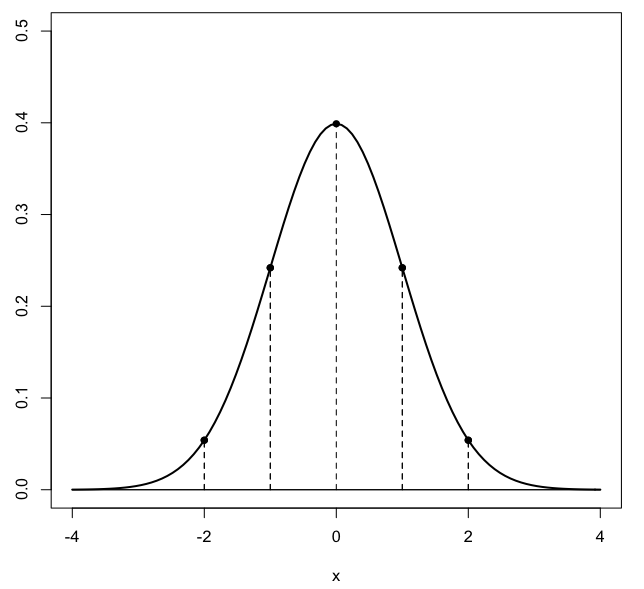
\includegraphics [scale=0.4] {gauss3.png} \end{center}

%break
\title{Line integral for work}
\date{}

\begin{document}
\maketitle
\Large

Here we extend the use of line integrals to calculate work moving along a curve in a field.  Review the \hyperref[sec:line_integrals]{\textbf{previous section}} on line integrals if you need to.

Suppose we have $x$ and $y$ as functions of a parameter $t$.  Also we may have a vector field $\mathbf{F}$ where
\[ \mathbf{F} = \langle \ M,N \ \rangle \]
or
\[ \mathbf{F} = \langle \ P,Q,R \ \rangle \]

It is usual to use $M,N$ in two dimensions and $P,Q,R$ in three.

We are interested in the integral along the curve (for the work done by $\mathbf{F}$):
\[ \int_C \mathbf{F} \cdot d\mathbf{r} = \int_C F \cdot \hat{\mathbf{T}} ds \]
\[ = \int_C P \ dx + Q \ dy + R \ dz \]

This last part seems like a magic trick.  We'll see how to justify it in the next section.  The crucial insight for evaluation is parametrization of the curve.  

\subsection*{example}

Suppose
\[ \mathbf{F} = \langle \ x,y,z \ \rangle \]
and we have equations for $x(t), y(t), z(t)$, say
\[ x = t, \ \ \ \ y = t, \ \ \ \ z = 2t^2 \]

Now,
\[ \mathbf{r}(t) = \ \langle x(t), y(t), z(t) \ \rangle \]
\[\frac{d\mathbf{r}}{dt} = \ \langle \ \frac{dx}{dt},\frac{dy}{dt},\frac{dz}{dt} \ \rangle \]
\[ = \ \langle \ 1,1,4t \ \rangle \]
Then
\[ \int_C \mathbf{F} \cdot d \mathbf{r} = \int \mathbf{F} \cdot \frac{d\mathbf{r}}{dt} \ dt \]
\[ = \int_C \ \langle \ t,t,2t^2 \ \rangle \  \cdot \ \langle \ 1,1,4t \ \rangle \ dt \]
\[ = \int_C (2t + 8t^3) dt = t^2 + 2t^4 \]
Evaluate from say, $t=0$ to $t=1$
\[  t^2 + 2t^4 = 3 \]
It doesn't seem complicated at all, once we have the parametric equations.

\subsection*{theory}

The basic line integral is something like this one for work
\[ W = \int_C \mathbf{F} \cdot d\mathbf{r} \]
We have a curve $C$ made up of lots of little pieces $d\mathbf{r}$.  For each piece, we compute the dot product with the force $\mathbf{F}$, multiplying by the component of the force that is in the same direction as we're headed.  

It makes great sense symbolically, but how to compute it?  Again

\[\frac{d\mathbf{r}}{dt} = \ \langle \ \frac{dx}{dt},\frac{dy}{dt},\frac{dz}{dt} \ \rangle \]

\[  \int_C \mathbf{F} \cdot d\mathbf{r} =  \int_C \mathbf{F} \cdot \ \langle \ \frac{dx}{dt},\frac{dy}{dt},\frac{dz}{dt} \ \rangle \ dt \]

If $\mathbf{F}$ has components
\[ \mathbf{F} = \ \langle \ P,Q,R \ \rangle \]
then this becomes
\[  \int_C  \ \langle \ P,Q,R \ \rangle \ \cdot \ \langle \ \frac{dx}{dt},\frac{dy}{dt},\frac{dz}{dt} \ \rangle \ dt \]
We could even write this
\[  \int_C  P \ dx + Q \ dy + R \ dz \]

This is a useful mnemonic to remember, but keep in mind that this is a single integral, we can't just do $dx$ and $dy$ separately.  We need a single variable and $t$, the parameter for the curve $C$, comes to the rescue.  (Either that or express $y$ and $z$ as functions of $x$.  We must get all these in terms of $t$.  Then it's OK.

Auroux uses the vector $\mathbf{\hat{T}}$.

\[ d\mathbf{r} = ds \ \hat{\mathbf{T}} \]

$\mathbf{\hat{T}}$ is the unit vector in the (tangential) direction of $d \mathbf{r}$, the direction the point (or particle or test mass or test charge) is moving at the moment ($d \mathbf{r}/dt$ is the velocity).  $ds$ is the magnitude of $d\mathbf{r}$.

Then
\[ \frac{d\mathbf{r}}{dt} = \mathbf{v} = \frac{ds}{dt} \ \hat{\mathbf{T}} \]
and 
\[ \frac{ds}{dt} \ \hat{\mathbf{T}} = \frac{dx}{dt} \ \mathbf{\hat{i}} + \frac{dy}{dt} \ \mathbf{\hat{j}} + \frac{dz}{dt} \ \mathbf{\hat{k}} \]
so
\[  \int_C \mathbf{F} \cdot d\mathbf{r} =  \int_C \mathbf{F} \cdot \mathbf{v} \ dt \]
\[ =  \int_C \mathbf{F} \cdot \ \frac{ds}{dt} \  \mathbf{\hat{T}} \ dt  \]
\[ =  \int_C \mathbf{F} \cdot \ [ \ \frac{dx}{dt} \ \mathbf{\hat{i}} + \frac{dy}{dt} \ \mathbf{\hat{j}} + \frac{dz}{dt} \ \mathbf{\hat{k}} \ ]  \ dt  \]
\[ =  \int_C \mathbf{F} \cdot \ [ \ dx \ \mathbf{\hat{i}} + dy \ \mathbf{\hat{j}} + dz \ \mathbf{\hat{k}} \ ]  \]
\[ = \int_C P \ dx + Q \ dy + R \ dz \]

\subsection*{example}

It may be necessary to break the curve up into pieces.
Suppose we're in $\mathbb{R}^2$ 
\[ \mathbf{F} = \ \langle x,y \rangle \ \]

Let $C$ be the unit square.  \textbf{This relationship provides the parametrization}.

For the first leg we have $x$ ranging from $0 \rightarrow 1$ and $y=0$.  So parametrize $x$ using $t$ by setting $x=t$ and let $t=0 \rightarrow 1$.

The integral is
\[ = \int_C M \ dx + N \ dy \]
\[ = \int_C x \ dx + y \ dy \]
\[ = \int_0^1 x \ dx = \frac{1}{2} \]

We could parametrize to $x = t$ here but we don't need to.

We can't just look at the field $\mathbf{F} = \ \langle x,y \rangle$ and substitute the parameter, unless we know the curve.

In a similar way, on the second leg (up to $(1,1)$), $x=1$ and $y$ ranges from $0 \rightarrow 1$, but notice that even though $x \ne 0$, $dx$ is zero.

\[ = \int_C x \ dx + y \ dy \]
\[ = \int_0^1 y \ dy = \frac{1}{2} \]

We have exactly the same integral.

For the third leg $y = 1$, $dy = 0$ and $x = 1 \rightarrow 0$ so
\[ = \int_C x \ dx + y \ dy \]
\[ = \int_1^0 x \ dx = - \frac{1}{2} \]

For the third leg $x = 0$, $dx = 0$ and $y = 1 \rightarrow 0$ so
\[ = \int_C x \ dx + y \ dy \]
\[ = \int_1^0 y \ dy = - \frac{1}{2} \]

 The total work is $1/2 + 1/2  - 1/2 - 1/2 = 0$.

That's interesting, why is the total work zero?  It turns out to be because our force $\mathbf{F} = \ <x,y>$ is the gradient of a potential function.  
\[ \mathbf{F} = \nabla \mathbf{f} \]
where
\[ \nabla = \ \langle \ \frac{\partial }{\partial  x},\frac{\partial }{\partial  y},\frac{\partial }{\partial  z} \rangle  \]
Can we guess what function? Sure!
\[ f(x,y) = \frac{1}{2}x^2 + \frac{1}{2}y^2 \]
That gives the correct values for the components of $\mathbf{F}$
\[ \mathbf{F} = \nabla \mathbf{f} = \nabla ( \frac{1}{2}x^2 + \frac{1}{2}y^2) \]
\[ = \ \langle  f_x,f_y \rangle  \ = \ \langle  x,y \rangle  \]
and since 
\[  \hat{\mathbf{T}} \ ds = (dx\ \hat{\mathbf{i}} + dy\ \hat{\mathbf{j}}) \]
Then, at least in the case where this gradient condition holds, we have

\[ \int_C \mathbf{F} \cdot  \hat{\mathbf{T}} \ ds  =  \int \ \langle  f_x,f_y \rangle  \  \cdot  (dx\ \hat{\mathbf{i}} + dy\ \hat{\mathbf{j}})  \] 
written with the "del" notation
\[= \int (\frac{\partial f}{\partial  x} \hat{\mathbf{i}} + \frac{\partial f}{\partial  y} \hat{\mathbf{j}}) \cdot (dx\ \hat{\mathbf{i}} + dy\ \hat{\mathbf{j}}) \]
\[ =\int \frac{\partial f}{\partial  x} \ dx + \frac{\partial f}{\partial  y} \ dy \]
\[ = \int df = f(\mathbf{r}_2) - f(\mathbf{r}_1)  \]

\subsection*{another example}
Suppose $\mathbf{F}$ is $\langle y,x \rangle $ and we want

\[ \int_C \mathbf{F} \cdot  d \mathbf{r} = \int_C M \ dx + N \ dy \]
\[ = \int_C y \ dx + x \ dy \]

$C$ is a sector of the unit circle between $0 <= \theta <= \pi/4$.  We break the curve up into 3 parts.

$\circ \ \ \ $ $C_1$ is from $(0,0)$ to $(0,1)$.  

$\circ \ \ \ $ $C_2$ is from $(0,1)$ to $(1/\sqrt{2},1/\sqrt{2})$. 

$\circ \ \ \ $ $C_3$ is from $(1/\sqrt{2},1/\sqrt{2})$ to $(0,0)$.  

For $C_1$, as before, notice that $y=0$, and $dy=0$ so 
\[ \int_C y \ dx + x \ dy = 0 \]
Also, notice that $\mathbf{F}$ is $\langle 0,x \rangle$, so $\mathbf{F} \perp d\mathbf{r}$ and then of course $\mathbf{F} \cdot d\mathbf{r} = 0$.

For $C_2$ from $(0,1)$ to $(1,0)$  Here, we're on the unit circle.  It's natural to change variables:

\[ x = \cos \theta \]
\[ dx = -\sin \theta \ d \theta \]
\[ y = \sin \theta \]
\[ dy = \cos \theta \ d \theta \]

\[ \int_C y \ dx + x \ dy  \]
\[ = \int_C -\sin^2 \theta \ d \theta + \cos^2 \theta \ d \theta \]
\[ = \int_C \cos \ 2 \theta \ d \theta \]
\[ = \frac{1}{2} \sin \ 2 \theta \ \bigg|_0^{\pi/4} = \frac{1}{2} \]

For $C_3$ from $(1/\sqrt{2},1/\sqrt{2})$ back to $(0,0)$, both $x$ and $y$ will change along the path, and we do need to parametrize in some fashion.  One way is
\[ x = t \ \ \ y = t \]
another way is
\[ x = y \]

If we just use $x=y$ and $dx=dy$ then
\[ \int_C y \ dx + x \ dy  \]
\[ 2 \int_C x \ dx \]
\[ = x^2  \ \bigg|_{1/\sqrt{2}}^0 = - \frac{1}{2} \]

So, once again, the total integral is $0$.

And the reason is that $\mathbf{F}$ is (again) the gradient ($\nabla$) of a potential function.  

By guessing, we obtain this formula for the potential:

\[ f(x,y) = xy \]
\[ F = \nabla f = \ \langle f_x,f_y \rangle \ = \ \langle y,x \rangle \]

The fundamental theorem of calculus for line integrals:

 \[ \int_C \nabla f \cdot d \mathbf{r} =   f(P1) - f(P2) \]
  
The example is a closed curve (P1 = P2), so of course it's just 0.  

But we can also do each part separately using the method.  We get $f(x,y) = (1/\sqrt{2} \times 1/\sqrt{2}) = 1/2$ along $C_2$ (starting from $0$ at $C_1$), and of course, minus that along $C_3$, back to $(0,0)$.

In the case where $\mathbf{F}$ is the gradient ($\nabla$) of a potential function
\[ \mathbf{F} \cdot d\mathbf{r} = (f_x \ \hat{\mathbf{i}} + f_y \ \hat{\mathbf{j}}) \cdot (dx \ \hat{\mathbf{i}} + dy \ \hat{\mathbf{j}} ) \]

The property that is required for $\mathbf{F}$ to be the gradient of a potential function $f$:
\[ \mathbf{F} = \nabla f = \langle f_x, f_y \rangle \]
is that the mixed second derivatives must be equal.  That is, if $\mathbf{F} = \langle M, N \rangle$, then
\[ M_y = N_x \]
is both necessary and sufficient for the force to be the gradient of a potential, for the force to be conservative, and for us to be able to evaluate the integral for work by just subtracting the value of the potential at the two endpoints.

In the language of \hyperref[sec:green]{\textbf{vector calculus}}, this requirement is the same thing as saying that the "curl" of the field must be zero, where curl $F = N_x - M_y$.

Shankar:

\begin{quote}We are beginning to see why certain integrals do not depend on the path. Here is an analogy. Forget about integrals. Imagine I am on some hilly terrain. I start at one point, and I walk to another point. At every portion of my walk, I keep track of my change in altitude, with uphill as positive and downhill as negative. That is like my dU. I add them all up. The total height change will be the difference in the heights of the end points. 

Now, you start with me but go on a different path. You wander all over the place but finally stop where I stopped. If you kept track of how long you walked, it won't be the same as my walk. But if you also kept track of how many feet you climbed at each step and added them all up, you would get the same answer I got. I repeat: if what you were keeping track of was the height change in a function, then the sum of all the height changes will simply be the height at the end minus the height at the beginning, independent of the path.\end{quote}.

There is finally, the issue of sign.  In the case of gravitation, the force points toward the earth (or whatever body we are talking about).  If we define positive as up, then the force is negative but the potential function is positive --- potential energy increases as we go away from the earth.  The upshot of this is that in physics the force and the potential have this relationship:
\[ \mathbf{F} = - \nabla U = - \langle U_x, U_y \rangle \]

\end{document}